
\section{Implementasi Algoritma Paralel pada Library big integer}
\subsection{Lingkungan Implementasi}
Sesuai dengan pertimbangan pada subbab \ref{sec:parallel_env}, implementasi algoritma paralel akan dilakukan dengan menggunakan pthread. Implementasi akan dilakukan menggunakan \textit{compiler} GCC versi 5.4.0 dan dijalankan pada sistem operasi Ubuntu 18.04 64-bit. Penggunaan TLS akan diuji pada penggunaan HTTPS pada web server yang diinstall pada sistem operasi. Web server yang digunakan adalah Apache2 dengan menggunakan modul tambahan mod\_ssl. Arsitektur sistem yang digunakan dapat dilihat pada Gambar \ref{fig:openssl_arch}

\begin{figure}[h]
  \centering
  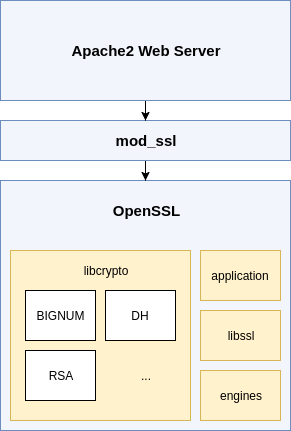
\includegraphics[width=0.4\textwidth]{resources/ch-4/implementation_arch.png}
  \caption{Arsitektur OpenSSL}
  \label{fig:openssl_arch}
\end{figure}

% Cek lagi jumlahnya
Secara default, jumlah maksimal thread maksimum yang akan digunakan oleh OpenSSL untuk menjalankan komputasi big integer secara paralel akan bergantung pada jumlah core yang terdapat pada lingkungan instalasi. Dalam aplikasi yang membutuhkan komputasi yang tinggi setiap thread akan berjalan secara terus menerus. Dengan demikian jumlah thread maksimum akan sama dengan jumlah aplikasi. Namun, aplikasi juga memiliki pilihan konfigurasi untuk menentukan jumlah thread maksimum yang dapat digunakan.
% \todo{cite disini}

\subsection{Batasan Implementasi}
Implementasi dilakukan pada sistem operasi Ubuntu 64 bit. Karena itu, implementasi library big number hanya berfokus pada openssl dengan yang memiliki konfigurasi makro sebagai berikut:
\begin{itemize}
  \item BN\_ULONG = unsigned long long
  \item OPENSSL\_SMALL\_FOOTPRINT = false
  \item BN\_MUL\_COMBA = true
  \item BN\_RECURSION = true

\end{itemize}

Konfigurasi makro tersebut digunakan dalam pemilihan dan manajemen struktur data yang digunakan serta pemilihan algoritma pada bagian tertentu. Sebagai contoh, algoritma yang digunakan dalam perkalian adalah algoritma karatsuba dan algoritma comba pada basis rekursif.

\subsection{Struktur Data Big Integer} \label{sec:bignum_struct}
Pada OpenSSL, sebuah big integer direpresentasikan dalam struktur data BIGNUM. BIGNUM terdiri dari sebuah array dengan ukuran dinamis dan beberapa integer yang menyimpan informasi tambahan. Dengan demikian secara teori BIGNUM tidak memiliki nilai maksimum. Untuk keperluan paralelisasi, BIGNUM dapat digunakan tanpa mengubah strukturnya sedikitpun. BIGNUM sendiri merupakan sebuah \textit{struct} yang memiliki deklarasi sebagai berikut.

\begin{lstlisting}[style = code]
struct bignum_st {
       BN_ULONG *d;
       int top;
       int dmax;
       int neg;
       int flags;
};
\end{lstlisting}

|BN_ULONG| sendiri adalah sebuah makro yang menggantikan |unsigned long| pada komputer 32 bit atau |unsigned long long| pada komputer 64 bit.

|d| adalah pointer untuk array of integer.

|top| merupakan index |d| yang terakhir digunakan plus satu.

|dmax| adalah panjang maksimum array yang telah dibuat. |neg| bernilai satu jika BIGNUM bernilai negatif.

% BIGNUM telah memiliki beberapa fungsi primitif yang dapat digunakan untuk membuat, memanipulasi, dan menghancurkan \textit{struct} tersebut. Primitif yang ada adalah seperti berikut.
%
% \begin{lstlisting}[style = code]
%  BIGNUM *BN_new(void);
%  void BN_init(BIGNUM *);
%  void BN_clear(BIGNUM *a);
%  void BN_free(BIGNUM *a);
%  void BN_clear_free(BIGNUM *a);
% \end{lstlisting}
%
% |BN_new()| akan mengalokasi dan menginisialisasi sebuah struktur BIGNUM.
%
% |BN_init()| menginisialisasi BIGNUM yang sudah ada.
%
% |BN_clear()| mengubah nilai seluruh komponen BIGNUM a (d, top, dmax) menjadi 0. |BN_clear()| dapat digunakan untuk menghapus data sensitif yang sudah tidak digunakan lagi seperti nilai kunci RSA atau AES.
%
% |BN_free()| mengembalikan memori komponen BIGNUM pada sistem.
% operand
% |BN_clear_free()| mengubah nilai seluruh komponen BIGNUM a menjadi 0 kemudian mengembalikan memori BIGNUM pada sistem.

% Sebutin fungsi yang dipake?
\subsection{Modul Operasi Aritmatika}
\subsubsection{Modul Penjumlahan}
Modul penjumlahan dan pengurangan terdapat pada file BN\_add.c. Fungsi BN\_add(result, a, b) pada modul ini melakukan pengolahan data pada a dan b seperti mengecek negatif dan mengecek panjang masing-masing array. Hasil pengecekan tersebut akan digunakan untuk melakukan operasi lebih lanjut. Jika a dan b memiliki tanda yang berbeda, akan dipanggil fungsi BN\_usub() selain itu akan dipanggil fungsi BN\_uadd(). BN\_uadd() dan BN\_usub() melakukan pengolahan data pada a dan b sehingga terdapat representasi array yang dapat diolah oleh BN\_add\_words() dan BN\_sub\_words().

BN\_add\_words merupakan fungsi yang menerima masukan dua array dengan ukuran yang sama dan menjumlahkannya secara sekuensial. Penerapan algoritma \ref{alg:add} pada OpenSSL terdapat pada fungsi ini.

% Paralelisasi dilakukan pada pemanggilan fungsi BN_add_word() oleh BN_uadd(). \todo{ini masukin kode? banyak banget? Kalo snippet ga ada context}
%
% \begin{lstlisting}
%     //rp -> result array, ap & bp original array, n length of ap & bp
%
%     a_split = split_array(ap, n);
%     b_split = split_array(bp, n);
%
%     ...
%
% \end{lstlisting}



\subsubsection{Modul Pengurangan}
\subsubsection{Modul Perkalian}
\subsubsection{etc.}
